\section{Optimal MP Problem}

In the previous section we developed the New Keynesian DSGE model, and explored its strengths and
weaknesses. While it isn't perfect, it's the best tool we have when it comes to understanding macroe-
conomics fluctuations, and to explain the business cycle data that we observe. More importantly, the
New Keynesian model allowed us to integrate a role for policy - most notably monetary policy - into
a macroeconomic DSGE model framework.

\subsection{What should monetary policy aim for?}

In this section, we will explore the implications of the New Keynesian model for monetary policy.

First, let's take a look at the considerations:

\begin{itemize}
    \item Menu costs: keep inflation at 0 to minimize costs
    \item Incomplete indexation of taxes: when households have to pay taxes on nominal income(labor, capital),
    an increase in inflation migh tpush them into a higher tax bracket, which distorts incentives. 
    So, monetary policy should target zero inflation.
    \item Zero lower bound for nominal interest rates: targeting positice inflation rates leaves more space to
    decrease $i$ during a recession.
    \item Measured inflation may overstate actual inflation due to
    incomplete adjustment for quality improvements, then the policy should target positive measured inflation.
    \item Nominal wages do not adjust downwards: target positive
    average inflation to allow real wages to fall in times of low TFP.
\end{itemize}

\underline{\textbf{Output/Unemployment Stabilization}}
Think of unemploymnet as inversely moving with output gap.
More careful analysis of unemployment wouls require modeling the labor market.

Triying to bring output up to the efficient level $\Leftrightarrow$ closing the output gap

But can we push output above the steady-state (= natural) level?

\begin{note}
    \

    Natural level $y_t^*$ < Efficient level $\hat{y}_t$
\end{note}

\subsection{Loss Function}
Choice for CB's optimal MP policy would be to maximize welfare, i..e the \textit{net present value} of 
expected utility of households, subject to the optimal responses and market conditiond of the model.

Woodford (2003) showed that the optimal policy can be expressed as a loss function:
\[L_t = \frac{1}{2} \left( (\tilde{\pi_t} - \pi^*)^{2} + a(\tilde{x_t} - x^*)^2 \right)\]
where notation as NKPC: everything in pct deciations form steady state, $\pi^*$ and $x^*$ are inflation and output gap targets.

Assume that CB cannot commit to a policy, i.e. chooses current period monetary policy only.

Then, optimal MP problem is:
\begin{align*}
    \min_{i_t} L_t &= \frac{1}{2} \left( (\tilde{\pi_t} - \pi^*)^{2} + a(\tilde{x_t} - x^*)^2 \right) \\
    \text{s.t.} \quad \tilde{\pi_t} &= \beta E_t \tilde{\pi}_{t+1} + \kappa \tilde{x_t} + u_t \\
    \tilde{x_t} &= \mathbb{E}_t(\tilde{x}_{t+1} + \sigma \tilde{\pi}_{t+1}) - \sigma \tilde{i_t} + v_t
\end{align*}

Interest rate it only features in IS curve, hence this problem is
equivalent to picking an output gap $\tilde{x_t}$ and omitting IS curve.

Straight forward solve for optimal $\tilde{x_t}, \tilde{\pi_t}$, we get:
\[\kappa(\tilde{\pi_t} - \pi^*) + a(\tilde{x_t} - x^*) = 0\]
with NKPC to find $\tilde{x_t}$ and $\tilde{\pi_t}$, and then use IS to find $i_t$.

\subsubsection{Conclusions}
\begin{itemize}
    \item When the economy is hit by shocks to the efficient real
    interest rate (such as TFP shocks), the CB should just move
    nominal interest rate accordingly so that the shock cancels
    out in the IS curve, \textit{There's no tradeoff for CB, it can stabilize
    both inflation adn output gap.};
    \item When the economy is hit by \textit{cost-push shocks}, 
    the CB faces a tradeoff that is given by the NKPC.
    Tradeoff becomes worse when inflation expectations $\mathbb{E}_t \tilde{\pi_t}$
    are high or cost-push shock $e_t$ is high (NKPC shifts up)
\end{itemize}

\subsection{Central Banks' Preferences}
Parameter $a$ governs the implrtance of output gap stabilization.
\begin{itemize}
    \item Hawkish CB: $a = 0$, CB only cares about inflation; $\var(x)$ is large , $\var(\pi)=0$
    \item Dovish CB: $a = \infty$, CB only cares about output gap; $\var(x)=0$, $\var(\pi)$ is large
\end{itemize}
If $\var(x) = \mathbb{E}X^2$ if $\mathbb{E}X = 0$.

If the CB minimizes the loss function Lt in every period and
implements the solution, this is called \textit{optimal monetary policy
under discretion.}

\subsection{Inflation bias}
Suppose CB chooses $\pi ^* = 0$ but $x^* > 0$ in every period.
Assume no shocks:
\[\min_{i_t}L_t = \frac{1}{2} \left(\pi_t^2 + a(\tilde{x_t} - x^*)^2\right)\]
the FOC is:
\[\tilde{x_t} = x^* - \frac{\kappa}{a}\pi_t,\]
the NKPC is:
\[\tilde{\pi_t} = veta\mathbb{E}_t \tilde{\pi}_{t+1} + \kappa\tilde{x_t}. \]
Plug in the recursive NKPC,
\[\tilde{\pi_t} = \mathbb{E}_t \sum_{j=0}^{\infty }\beta^j \kappa \tilde{x}_{t+j} \]
we get:
\[\tilde{\pi_t} = \frac{\kappa}{1-\beta} x^* - \mathbb{E}_t \sum_{j=0}^{\infty}\beta^j \frac{\kappa^2}{a} \pi_{t+j}. \]
In this case, we need to solce the expectations of future variables.

Note that in the next period, the CB's problem will look exactly like in
this period. Hence optimal solution must be the same in all periods $\pi_t = \bar{\pi}$
for all $t$. Because of rational expectations:
\[\tilde{\pi_t} = \mathbb{E}_t \tilde{\pi}_{t+1} = \bar{\pi}. \]
Solving the $\pi_t$ above, we get:
\[\tilde{\pi_t} = \bar{\pi} = \frac{\kappa}{1-\beta + \frac{\kappa^2}{a}}x^*,\]
hence
\[\tilde{x_t} = x^* - \frac{\kappa}{a} \frac{\kappa}{1-\beta + \frac{\kappa^2}{a}}x^*.\]

How large are these magnitudes? For $\beta \to 1$,
\[\lim_{\beta \to 1} \tilde{x_t} = 0, \quad \lim_{\beta \to 1} \tilde{\pi_t} - \frac{a}{\kappa}x^*\]
Hence $\tilde{x_t}$ is close to 0 but $\pi_t$ is positive,meaning that we are away from the target!

\subsection{Optimal monetary policy with commitment}
Instead of re-optimizing every period, the CB could plan a MP rule
(a set of $\{i_t\}_t$ contingent on shocks). This would generally lead to
a preferable outcome, called “commitment,” the CB solves the entire problem at the beginning of time and commits to its policy.

Here, the objective of the central bank is not just the current objective, 
but the present discounted value of the flow objective functions. 

Let's consider a simple scenario: $x^* = \pi ^* = 0$, with positive cost-push shock $e_t > 0$,
but short-lived $\mathbb{E}_t e_{t+j} = 0$ for $j>0$, assume we are at time 0.
The problem for the central bank is
\begin{align*}
    \min_{\{\pi_t\}, \{x_t\}} & L = \frac{1}{2} \mathbb{E}_0 \sum_{t=0}^{\infty} \beta^t \left(\tilde{\pi_t}^2 + a \tilde{x_t}^2\right) \\
    \text{s.t.}\quad & \tilde{\pi_t} = \beta \mathbb{E}_t \tilde{\pi}_{t+1} + \kappa \tilde{x}_t + e_t \text{ for every time period}
\end{align*}
Define the Lagrangian:
\[\mathcal{L} = \mathbb{E}_0 \sum_{t=0}^{\infty} \beta^t \left(\frac{1}{2} \left(\tilde{\pi_t}^2 + a\tilde{x_t}^2\right) + \lambda_t \left(\tilde{\pi_t} - \beta \mathbb{E}_t \tilde{\pi}_{t+1} - \kappa \tilde{x}_t - e_t\right) \right) \]
Take FOCs(w.r.t. $\tilde{\pi}_{t+1}, \tilde{x_t}$):
\begin{align*}
    \frac{\partial \mathcal{L}}{\partial \tilde{\pi}_{t+1}} &= \beta (\tilde{\pi}_{t+1} + \lambda_{t+1}) - \beta\lambda_{t}= 0 \\
    \frac{\partial \mathcal{L}}{\partial \tilde{x_t}} &= a\tilde{x_t} - \kappa \lambda_t = 0
\end{align*}

Note that the NKPC at time -1 is not a restriction, hence FOC for $t=0$ is:
\[\tilde{\pi_0} + \lambda_0 = 0\]
and we can eliminate $\lambda_t$ to solve for $\tilde{x_t}$ and $\tilde{\pi_t}$:
\begin{align*}
    \tilde{x_t} - \tilde{x}_{t-1} &= -\frac{\kappa}{a} \tilde{\pi_t} \\
    \tilde{x_0} &= -\frac{\kappa}{a} \tilde{\pi_0}
\end{align*}

\subsection{Time consistency of the policy}
\begin{itemize}
    \item The optimal monetary policy with commitment features
    history dependence, i.e. policy decision for period $t$ depends
    on what we want to implement in period $t-1$.
    \item Exception: optimal policy for period 0 does not depend on
    past (why? economy is only forward-looking)
    \item The optimal policy with commitment is time inconsistent:
    at time 0, what we want to implement for period 1 is not what 
    we will want to implement for period 1 at time 1.
\end{itemize}

\begin{figure}[!htbp]
    \centering
    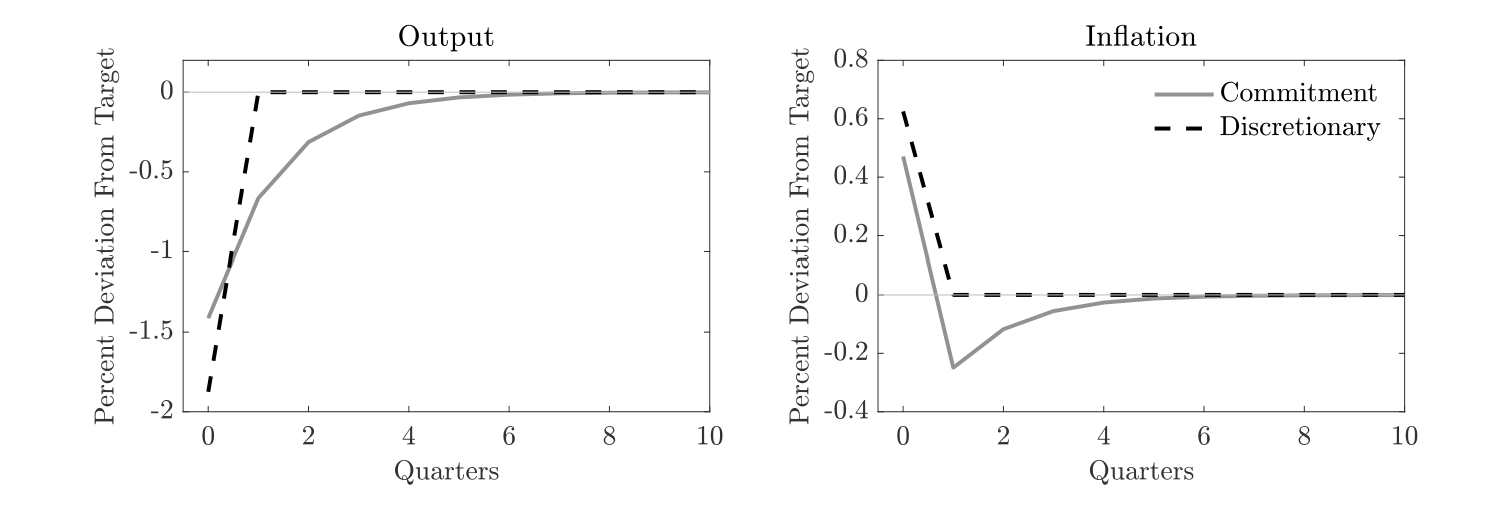
\includegraphics[width=0.8\textwidth]{figures/OptPolicy.png}
    \caption{Response of output and inflation to a transitory cost push shock
    under commitment and discretionary policies.}
    \label{fig:241111_1}
\end{figure}

\begin{remark}
    \

    While the outcomes from the commitment policy are better than those from the discretionary policy at date 0, 
    they are worse at future dates. Under the discretionary policy, there are no deviations in output or inflation at any date $t \geq 1$ while, 
    under the commitment policy, output and inflation are too low relative to the targets. 
    
    This brings us to a \textcolor{blue}{\textit{time-consistency problem.}}
    
    At date 0, the central bank would like to announce the commitment policy, 
    but it would like to switch to the discretionary policy at date 1. 
    If the private sector anticipates this switch in policy, 
    then the benefits of the commitment policy at date 0 are unattainable 
    because the central bank cannot convince the private sector that $\pi_1$ will be negative. 
    
    The central bank can only achieve the better outcomes if 
    it is able to commit at date 0 to have tight monetary policy at future dates even though 
    it will not want to do that when those future dates arrive.

    Under the \textcolor{blue}{\textit{discretionary policy}}, 
    the price-level jumps at date 0 and then remains constant thereafter.

    Under the \textcolor{blue}{\textit{commitment policy}}, the price level rises, 
    but then falls subsequently as inflation is negative for several periods. 
    In fact, if you accumulate the inflation rates in the figure, 
    you find that the long-run price level is unaffected. 
    
    This result demonstrates that long-run price stability is useful for a central bank 
    even if it is pursuing an inflation targeting framework because it serves to stabilize inflation expectations 
    and therefore helps stabilize inflation rates.
\end{remark}

\subsection{What if the CB cannot observe everything?}
In reality, the CB faces uncertainties:
\begin{itemize}
    \item Shock uncertainty: $e_t$ is not directly observed;
    \item Parameter uncertainty: $\kappa$ not directly observed.
\end{itemize}
Pretty straightforward to study optimal policy problem with these
extensions in the linear-quadratic framework

\underline{Basic Outcomes:}

\begin{itemize}
    \item If there is uncertainty about something that enters additively
    (like shocks), the CB should ignore the uncertainty and act
    based on the expectation.
    \item If there is uncertainty about something that enters
    multiplicatively (like parameters in front of the variables), then
    the CB should do MP more cautiously (i.e. muted responses).
\end{itemize}